\documentclass[a4paper, 12pt]{article}
\usepackage{cmap}
\usepackage[utf8]{inputenc}
\usepackage[english, russian]{babel}
\usepackage[left=2cm, right=2cm, top=2cm, bottom=2cm]{geometry}
\usepackage{amsfonts,amssymb}
\usepackage{amsmath}
\usepackage{amsthm}
\usepackage{titlesec}
\usepackage{graphicx}
\usepackage{mathtools}
\usepackage{hyperref}

 \newcommand{\tit}[1]{\begin{center}{\bf{\Large #1}}\end{center}}
 \newcommand{\aut}[1]{\centerline{{\bf #1}}}
 \newcommand{\cityorg}[1]{\centerline{\it #1}}
 \newcommand{\email}[1]{\centerline{{\small e-mail: #1}}\vspace{\baselineskip}}
\providecommand{\keywords}[1]{\textbf{\textit{Ключевые слова:}} #1}
\newcommand{\norm}[1]{\left\lVert#1\right\rVert}
\newcommand{\normb}[1]{\left\lVert\textbf{#1}\right\rVert}

\begin{document}

\sloppy
 \tit{Маскировка при помощи оптимизированных однородынх анизотропных слоев}
 \aut{Bogdan-Ioan Popa, Steven A. Cummer}

\begin{abstract}
Мы представляем метод уменьшения рассеяния произвольных объектов, заключающийся
в окружении их оболочкой, состоящей из нескольких слоев анизотропных однородных 
материалов. Для нахождения материальных параметров для каждого слоя используется
оптимизаионный метод, отправной точкой которого является дискретная аппроксимация
координатного преобразования маскирующей оболочки. Мы покажем, что оптимизированная
трехслойная оболочка может снизить рассеяние на целых 15дБ больше, чем 100 слойная
реализация маскирующей оболочки с преобразованием координат. Более того,
оптимизационный метод может решения высокопроизводительной маскировочной оболочки,
которые удовлетворяют внешним ограничениям, таким как максимальное значение
диэлектрической или магнитной проницаемости. Такой подход может значительно
упростить маскировочных оболочек среднего размера. 
\end{abstract}

Недавно значительные исследования сфокусировались на разработке новых
методов оптимизации взаимодействия между заданными объектами и электромагнитыми
волнами. Пендри и другие \cite{1} показали, что тщательно спроектированные
неоднородные и анизотропные оболочки могут препятствовать распостранению
электромагнитного излучения внутрь них, и, гораздо важнее, убирает рассеяние
этих оболочек, превращая их и их внутренность прозрачным для электромагнитных волн.
В преобразовании координат является привлекательным его общность: 
он может быть применен для сокрытия объектов любой формы и размера.

Несмотря на то, что численное моделирование \cite{2} и далее теоретический анализ
\cite{3} подтвердили эффективность этого метода, эксперементальные демонстрации
оказались более сложной задачей. Одна попытка \cite{4}, включающая цилиндрическую
оболочку, окружающую металлический цилиндр продемонстировала основную физику
таких структур, а именно, что волны можно напрвлять вокруг структуры. Однако,
в данной работе были сделаны приближения \cite{2}, значительно снижающие
эффективность оболочки. В другой работе были выведены различные аппроксимации
к идеальной маскировочной оболочке, которые также жертвуют производительностью
в пользу простоты изготовления \cite{5}-\cite{7}.

Трудность построения маскировочных оболочек, заданных теорией преобразования
координат, вытекает из требований материала, их состовляющего: оболочка должна
быть анизотропной, с диэлектрической и магнитной проницаемостью непрерывно
изменяющимися в широком диапазоне значений. Физическая ее реализация 
всегда будет требовать некоторую форму дискретизации этих непрерывных профилей.
Например, Шуринг и другие \cite{4} в их эксперименте использовали десятислойную 
ступенчатую аппроксимацию идеальных параметров.

Начиная с идеи, что анизотропия, кажется, является самым важным ингридиентом
маскирующих оболочек, которые не являются электрически малыми, можно было бы
задаться вопросом, могут ли анизотпроные оболочки, состоящие из антизотропных 
слоев, построены другим образом? Здесь мы покажем, что уменьшающие рассение
оболочки, составленные из относительного малого числа однородных слоев,
могут быть построены при помощи оптимизаионного метода, использующего 
оболочку, построенную по принципу преобразования координат в качестве начального 
условия.
Производительность менее чем 5 оптимизированных слоев может быть равной,
или даже превосходить стослойную дискретную аппроксимацию гладной однородной
оболочки, построенной через преобразование координат.

Для простоты, мы сосредоточим наше внимание на двумерной цилиндрической оболочке
для элекромагнетизма, но представленный здесь анализ может быть применем для
других геометрий и типов волн, таких, как акустические \cite{8}. На рис. 1
изображен идеальный электрический проводник --- цилиндрический объект радиуса
$a$, окруженный оболочкой с внешним радиусом $b$. Было показано \cite{2},
что один набор относительных материальных параметров, который может полностью
убрать рассеяние от структуры имеет вид (в цилиндрических координатах):

\begin{equation*}
	\epsilon_r(r) = \mu_r(r) = \frac{r-a}{r}, \qquad 
	\epsilon_\phi(r) = \mu_\phi(r) = \frac{r}{r-a},
\end{equation*}

\begin{equation}\label{e1}
	\epsilon_z(r) = \mu_z(r) = \left( \frac{b}{b-a}	\right)^2 \frac{r-a}{r},
\end{equation}
где $z$ --- инвариантное направление, а $r$ и $\phi$ --- ридиальная и азимутальная
координаты соответственно.

Мы рассматриваем только поперечно электрическую поляризацию, для которой
релевантны только $\epsilon_z, \mu_r$ и $\mu_\phi$. Предполоаем, что оболочка
может быть собрана из $M$ концентрических слоев однородного материала, как показано
на рис. 1. Каждый слой характеризуется тензорами диэлектрической и магнитной
проницаемости, являющимися постоянными внутри слоя. Наша цель заключается в 
нахождении набора параметров, который бы минимизировал рассеяние оболочки.
Один способ --- использовать поваговое приближение \eqref{e1}, как в \cite{4}.
Используя этот подход и TE поляризацию, как было указано нами ранее \cite{9,10},
граничные условия на внутренней поверхности идеального проводника индуцируют
значительное рассеяние. Поэтому мы ожидаем, что другой выбор материальных 
параметров может улучшить производительность маскировки.

Далее предпологается $\exp(+jwt)$ соглашение по времени. Рассмотрим плоскую волну,
имеющую электрическое поле $E_{inc} = \hat{z}\exp(-jk_0r\cos\phi)$ падающую
на оболочку и объект, обозначенную на рис. 1. Симметрия задачи позволяет нам
внутри и вне нашей структуры аналитически, используя процедуру, обозначенную в
\cite{11}.

Таким образом, падающая волна может быть разложена в сумму функций Бесселя
первого рода как 

\begin{equation}
	E_{inc} = J_0(k_0r) + 2\sum\limits_{n=1}^\infty j^nJ_n(k_0r)\cos(n\phi),
\end{equation}
в то время как рассеянное поле в области $r > b$ может быть записано в терминах
функций Ханкеля второго рода следующим образом:

\begin{equation}
	E_{sc} = \sum\limits_{n=0}^\infty A_nH_n^{(2)}(k_0r)\cos(n\phi).
\end{equation}
Поля на слое $m$ внутри оболочки задаются соотношениями

\begin{equation}\label{e3}
	E_m = \sum\limits_{n=0}^\infty[B_{mn}J_v(k_mr) + C_{mn}Y_v(k_mr)]\cos(n\phi),
\end{equation}
где для всех $m=\overline{1,M},\; Y_n$ --- функция Бесселя второго рода,
$k_m=\omega\sqrt{\epsilon_{z,m}\mu_{\phi,m}}$ и $v=n\sqrt{\mu_{\phi,m}/\mu_{r,m}}$.
Коэффициенты $A_n, B_{mn}$ и $C_{mn}$ могут быть найдены из условия непрерывности
тангенциальных E и H полей вдоль границы на каждом уровне.

Как только мы знаем поля внутри и вне нашей структуры, мы можем измерить 
показатель качества, используемый в этой статье: эффективная поверхность
рассеяния на единицу длины, также известная как ширина рассеяния (SW),
которая определяется как $\sigma(\phi)=2\pi R|E_{sc}(\phi,R)/E_{inc}|^2$, здесь
$R$ --- расстояние от объекта, где было измерено далекое рассеянное поле $E_{sc}$.
Так как в дальней зоне $E_{sc}$ обратнопропорционально $R$, $\sigma$ независима
от $R$, пока оно достаточно большое.

Вопрос в том, можем ли мы получить набор материальных параметров для слоистой
оболочки, который бы уменьшал рассеяние больше, чем если бы мы просто
дискритезировали профили, заданные \eqref{e1}. Ответ положительны, и мы обозначим
процедуру для общего случая оболочки из $M$ слоев, после чего мы применим
метод на конкретном примере.

Чтобы максимально уменьшить видимость объекта, следует минимизировать 
$\max_\phi \sigma_\phi$. Однако, так как прямое рассеяние объекта, который не 
является электрически маленьким, как правило наибольшее \cite{12},
мы решаем простую задачу оптимизации тензоров диэлектрической и магнитной 
проницаемости, которая минимизирует прямое рассеяния (т.е. тень). Как мы увидим
далее, эта эвристика дает сильное уменьшение SW по всем направлениям.
Математически, мы хотим подобрать значения $\epsilon$ и $\mu$, которые 
минимизируют функцию $\sigma(\phi=0, \epsilon_z^{(1..M)}, \mu_r^{(1..M)}, 
\mu_\phi^{(1..M)}$, верхние индексы означают, что мы имеем один набор
материальных параметров для каждого из $M$ слоев. Эта классическая задача
оптимизации может быть решена множеством алгоритмов.
В этой работе мы исльзовали алгоритм Бройдена—Флетчера—Гольдфарба—Шанно (BFGS),
который уже реализован в програмных пакетах, таких как MATHEMATICA и MATLAB.
Метод BFGS находит локальный минимум для $f$ вокруг указанной начальной точки,
$X_0=(\epsilon_{z,0}^{(1..M)}, \mu_{r,0}^{(1..M)}, \mu_{\phi,0}^{(1..M)})$,
выбор которой очень существенен для успешности этого алгоритма.
Так как это уже дало хорошие результаты, $X_0$ выберем дискритезированной
версией \eqref{e1}, а именно, $\epsilon_{z,0}^{(i)}=\epsilon_z(r=[R_i+R_{i+1}]/2)$
(аналогичные выражения для $\mu_{r,0}^{(i)}$ и $\mu_{\phi,0}^{(i)}$), где
$R_i$ и $R_{i+1}$ --- внутрення и, соотвественно, внешняя слоя $i, \; R_1=a$ и
$R_{M+1}=b$. Локальный минимум в $\sigma(\phi=0)$ дает материальные параметры
для каждого из $M$ слоев.

Покажем процедуру для объекта, который имеет размеры, указанные в \cite{2},
тоесть $a=10$см, что делает его 1.33 длины волны на рабочей частоте 2ГГц.
Мы решили разработаь тонкую оболочку 1.3см, тоесть $b=11.3$см. Для этого 
размера, три слоя предоставляют достаточно степеней свободы (в сумме девять,
т.е. $\epsilon_z, \mu_r$ и $\mu_\phi$ дла каждого слоя) чтобы значительно
уменьшить ширину рассеяния нашего объекта. Таблица 1 показывает начальную точку
и материальные параметры, найденный опмизационным алгоритмом, а на рис. 2
показана  ширина рассеяния, нормированная к диаметру объекта, по отношению угла
для нашего построения (кривая d) и, для сравнения, три других наших оболочки,
профили материальных параметров которых есть три, девять и стоуровневые 
пошаговые аппроксимации \eqref{e1}.


Этот пример показывает, что метод оптимизации, представленный здесь,
не только позволяет нам проектировать оболочки, с уменьшенным количеством слоев,
но также значительно улучшить их производительность. В этом случае, максимальное
рассеянное поле приблизительно на 15дБ меньше для оптимизированно1 трехслойной
оболочки, чем для стослойной дискретизации оболочки, построенной при помощи
преобразования координат. Рис. 3 показывает вклад этих рассеянных полей в 
результуриющие поля: оптимизированная версия значительно меньше возмущает
входящее поле, что пошаговая аппроксимация аналитической оболочки.
Отметим также, что хотя $\mu_\phi=47$ на самом внутреннем слое оболочки
трудно достичь с текущими материалами, это по крайней мере значительно меньше,
чем для девятислойных ($\mu_\phi=139$) или для стослойных ($\mu_\phi=1539$)
ариближений аналитической оболочки.

С точки зрения чувствительности, случайные возмущения до 1\% примененные 
одновременно для всех оптимизированных $\epsilon$ и $\mu$ параметров,
указанных в таблице 1, изменили ширину рассеяния на $\pm5$дБ для большинства углов.
Это делает оптимизированную оболочку достаточно чуствительной к изменениями
в желаемых параметрах, но даже с этими возмущениями, производительность
оптимизированной оболочки значительно лучше, чем у дискретизированной
аналитической оболочки. Мы также подчеркиваем важность выбора хорошей
начальной точке в BFGS алгоритме. Если, например, вы выберем
компоненты начальных диэлектрической и магнитную проницаемости
равными единице, итоговые значения, полученные итерационным алгоритмом в оболочке
таковы, что хотя они и  уменьшают общее рассеяние, по сравнению с голым цилиндром,
но имеют максимальную ширину рассеяния на 30дБ больше, чем оптимальная оболочка,
определенная в таблице 1.

Процедура оптимизации, приведенная выше показывает, что для объекта диаметром
1.33 длины волны трехслойная оптимизированная оболочка более чем в сто раз 
лучше, чем трехслойная аппроксимация аналитической оболочки. Если мы 
удвоим размер объекта (т.е. 2.66 длины волны в диаметре), то улучшение будет
только в 7 раз. Еще раз умножив на 2 (т.е. 5.32 длины волны) улучшение
проищойдет только в два раза. Эта зависимость улучшения оптимизации от
размера ожидаема, когда объект становится больше, нам требуется 
минимизировать все больше коэффициентов в разложении рассеянного поля \eqref{e3}.
Три слоя не обеспечивают достаточное количество степеней свободы, чтобы
резко улучшить маскировку объекта шириной 5 длин волы. Однако, увеличивая
количество слоев, мы ожидаем значительные улучшения в оптимизации 
больших объектов.

Оптимизация дает большую гибкость в ограничениях, которые могут быть наложены на
маскирующие оболочки. Уравнение \eqref{e1} показывает, что для тонких оболочек
требуемое значение $\mu_\phi$ на самом внуреннем слое должно быть большим (
в предыдущем примере оно равнялось $\mu_\phi=47$), что может стать
препятствием для производства. Эти предельные значения могут быть уменьшены
оптимизацией и все еще давайть значительное улучшение по сравнению с 
дискретизированной аналитической оболочкой. Мы покажем это на следующем примере,
разработав немагнитную оболочку, которая потенциально может применятся
на видимых частотах.

С практической точки зрения, несмотря на то, что оболочка, описанная выше, требует только три слоя, ее трудно построить: требуется одновременно и 
$\epsilon$ и $\mu$, к томуже, эти параметры должны быть достаточно большими
(например $\mu_\phi$ должно быть равным 47 на самом внутренннем слое), чего сложно
достичь на больших частотах. По этой причине, большой интерес предаставляет 
собой разработка маскирующей оболочки с заданными свойствами, которую легко
сконструировать. Некоторые приближения к идеальным параметрам были исследованы 
\cite{2,5} в целях облегчения физической реализации, но большинство из
них в большей степени жертвуют производительностью.

Одним из таких наборов параметров, которые избегают трудности построения
магнитных материалов, и могут быть использованы для создания оболочек,
которые могут скрытьвать объекты от обнаружения TM поляризованными волнами
(для этой реализации релевантны только $\mu_z, \epsilon_r$ и $\epsilon_\phi$)
является следующий

\begin{equation}\label{e5}
  \epsilon_r = \left( \frac{b}{b-a} \right)^2 \left( \frac{r-a}{r}\right)^2,
  \qquad
  \epsilon_\phi = \left( \frac{b}{b-a}\right)^2,
  \qquad
  \mu_z =1.
\end{equation}

Рассматривая тот же объект, что и раньше (т.е. $a=10$см), рис 4
показывает ширину рассеяния в зависимости от угла, $\sigma(\phi)$,
для относительно тонкой маскировочной оболочки с внешним радиусом $b=17$см
состощая из среды, параметры которой задаются уравнением выше (пунктирная кривая),
по сравнению с трехслойной аппроксимацией аналитиеской оболочки (пунктирно-точечная
кривая). Мы выбрали более тонкую оболочку, по сравнению с предыдущей
чтобы получить более достижимые материальные параметры внутри. Ни одна из
этих аппроксимаций не достигает особенно хорошей производительности.

Оптимизация может резко улучшить производительность трехслойной немагнитной
оболочки. Начальное предположение задается \eqref{e5} и мы добавили дополнительное ограничение для упрощения производства, что ни одна компонента диэлектрической
или магнитной проницаемости не может быть больше 10. Результирующией
оптимизированные материальные параметры представлены в таблице 2, а
вычисленная ширина рассеяния на рис. 4. Эта оптимизированная трехслойная оболочка
дает приблизительно 15дБ уменьшения ширины рассеяния по сравнению с оболочкой,
описываемой \eqref{e5}, рис 4 (нижний) демонстрирует общее распределение
электрического поля вокруг оболочки и показывает ее хорошую производительность.
Отметим, что, как и ожидалось, более строгие требования по $\epsilon$ увеличивают
 $\sigma$ и, следовательно, уменьшают до некоторой степени производительность оболочки. Например, если мы требуем $\epsilon \le 5$, то $\max_\phi \sigma$
достигает 0 дБ, а для $\epsilon \le 8$, $\max_\phi \sigma \approx -5$дБ.

В заключение, мы представили практический оптимизационный подход, исопльзуемый для
построения слоей оболочки из анизотропныз материалов, которые значительно
уменшают ширину рассеяния объекта. Такой подход дает лучшую производительность
и может так же предоставлять более простые материальные параметры, в сравнении
с маскирующими оболочкам, построенными с помощью теории пробразования
координат. В качестве примера мы нашли, что оптимизированная трехслойная оболочка
может работать намного лучше, чем стослойная аппроксимация аналитической оболочки.
Мы также ипользовали этот подход для построения трехслойной немгнитной оболочки,
сделанной из анизотропных материалов, с относительно небольшой диэлектриечской
проницаемостью, реализуемы даже на оптических частотах, что значительно лучше,
чем сравнимые разработки.

\subparagraph*{Таблица 1.}

\begin{table}[h]
\begin{tabular}{lllllll}
\hline
\multicolumn{1}{|l}{}     & \multicolumn{3}{|l}{начальное предположение}                                                       & \multicolumn{3}{|l|}{оптимизированные параметры}                                                    \\ \hline
\multicolumn{1}{|l}{Слой} & \multicolumn{1}{|l}{$\epsilon_z$} & \multicolumn{1}{|l}{$\mu_r$} & \multicolumn{1}{|l}{$\mu_\phi$} & \multicolumn{1}{|l}{$\epsilon_z$} & \multicolumn{1}{|l}{$\mu_r$} & \multicolumn{1}{|l|}{$\mu_\phi$} \\ \hline
\multicolumn{1}{|l}{1}    & \multicolumn{1}{|l}{1.60}         & \multicolumn{1}{|l}{0.021}   & \multicolumn{1}{|l}{47.15}      & \multicolumn{1}{|l}{3.32}         & \multicolumn{1}{|l}{0.006}   & \multicolumn{1}{|l|}{47.21}      \\ \hline
\multicolumn{1}{|l}{2}    & \multicolumn{1}{|l}{4.61}         & \multicolumn{1}{|l}{0.061}   & \multicolumn{1}{|l}{16.38}      & \multicolumn{1}{|l}{6.06}         & \multicolumn{1}{|l}{0.039}   & \multicolumn{1}{|l|}{16.88}      \\ \hline
\multicolumn{1}{|l}{3}    & \multicolumn{1}{|l}{7.40}         & \multicolumn{1}{|l}{0.098}   & \multicolumn{1}{|l}{10.23}      & \multicolumn{1}{|l}{7.99}         & \multicolumn{1}{|l}{0.10}    & \multicolumn{1}{|l|}{10.63}      \\ \hline                                 
\end{tabular}
\end{table}

\subparagraph*{Таблица 2.}

\begin{table}[h]
\begin{tabular}{lllllll}
\hline
\multicolumn{1}{|l}{}     & \multicolumn{3}{|l}{начальное предположение}                                                            & \multicolumn{3}{|l|}{оптимизированные параметры}                                                         \\ \hline
\multicolumn{1}{|l}{Слой} & \multicolumn{1}{|l}{$\mu_z$} & \multicolumn{1}{|l}{$\epsilon_r$} & \multicolumn{1}{|l}{$\epsilon_\phi$} & \multicolumn{1}{|l}{$\mu_z$} & \multicolumn{1}{|l}{$\epsilon_r$} & \multicolumn{1}{|l|}{$\epsilon_\phi$} \\ \hline
\multicolumn{1}{|l}{1}    & \multicolumn{1}{|l}{1}       & \multicolumn{1}{|l}{0.064}        & \multicolumn{1}{|l}{5.90}            & \multicolumn{1}{|l}{1}       & \multicolumn{1}{|l}{0.10}         & \multicolumn{1}{|l|}{4.49}            \\ \hline
\multicolumn{1}{|l}{2}    & \multicolumn{1}{|l}{1}       & \multicolumn{1}{|l}{0.40}         & \multicolumn{1}{|l}{5.90}            & \multicolumn{1}{|l}{1}       & \multicolumn{1}{|l}{1.38}         & \multicolumn{1}{|l|}{9.99}            \\ \hline
\multicolumn{1}{|l}{3}    & \multicolumn{1}{|l}{1}       & \multicolumn{1}{|l}{0.80}         & \multicolumn{1}{|l}{5.90}            & \multicolumn{1}{|l}{1}       & \multicolumn{1}{|l}{0.70}         & \multicolumn{1}{|l|}{0.89}            \\ \hline
\end{tabular}
\end{table}
\begin{thebibliography}{99}
\bibitem{1}J. B. Pendry, D. Schurig, and D. R. Smith, Science 312, 1780 (2006)
\bibitem{2}S. A. Cummer, B.-I. Popa, D. Schurig, D. R. Smith, and J. B. Pendry, Phys. Rev. E 74, 036621 (2006).
\bibitem{3}H. Chen, B.-I. Wu, B. Zhang, and J. A. Kong, Phys. Rev. Lett. 99, 063903 (2007).
\bibitem{4}D. Schurig et al., Science 314, 977 (2006).
\bibitem{5}W. Cai et al., Appl. Phys. Lett. 91, 111105 (2007).
\bibitem{6}Y. Huang, Y. Feng, and T. Jiang, Opt. Express 15, 11133
(2007).
\bibitem{7}H. Ma et al., Opt. Express 16, 15449 (2008).
\bibitem{8}S. A. Cummer, B. I. Popa, D. Schurig, D. R. Smith, J. Pendry, M. Rahm, and A. Starr, Phys. Rev. Lett. 100, 024301 (2008).
\bibitem{9}Z. Ruan, M. Yan, C. W. Neff, and M. Qiu, Phys. Rev. Lett. 99,
113903 2007.
\bibitem{10}A. Greenleaf et al., Opt. Express 15, 12717 (2007).
\bibitem{11}C. A. Balanis, Advanced Engineering Electromagnetics
(Wiley, New York, 1989).
\bibitem{12}J. I. Glaser, IEEE Trans. Aerosp. Electron. Syst. AES-21, 70
(1985).
\end{thebibliography}

\clearpage 

\begin{figure}[t]
  \centering
  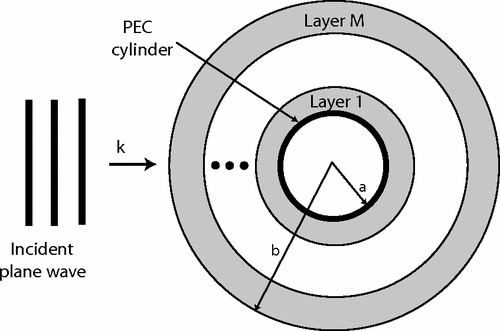
\includegraphics[height=0.25\paperheight, width=0.55\paperwidth]{fig1.png}
  \caption{Цилиндрический идеальный проводник, окруженный многослойной оболочкой
  и освещенный плоской волной. Входный и выходные радиусы оболочки есть 
  $a$ и $b$ соответственно.}
  \label{fig:1}
\end{figure}

\begin{figure}[t]
  \centering
  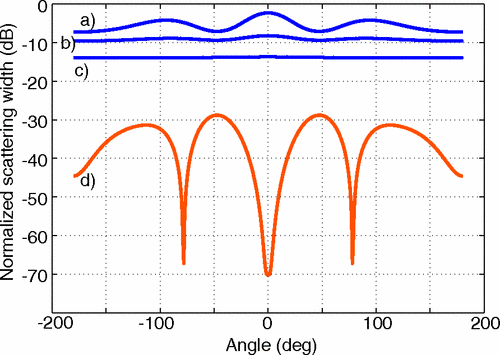
\includegraphics[height=0.25\paperheight, width=0.55\paperwidth]{fig2.png}
  \caption{}
  \label{fig:2}
\end{figure}

\begin{figure}[t]
  \centering
  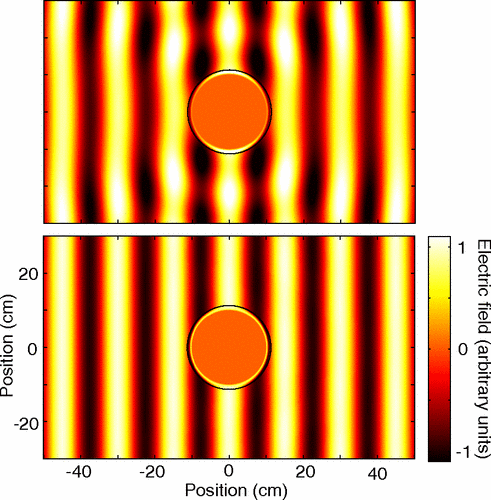
\includegraphics[height=0.4\paperheight, width=0.55\paperwidth]{fig3.png}
  \caption{}
  \label{fig:3}
\end{figure}

\begin{figure}[t]
  \centering
  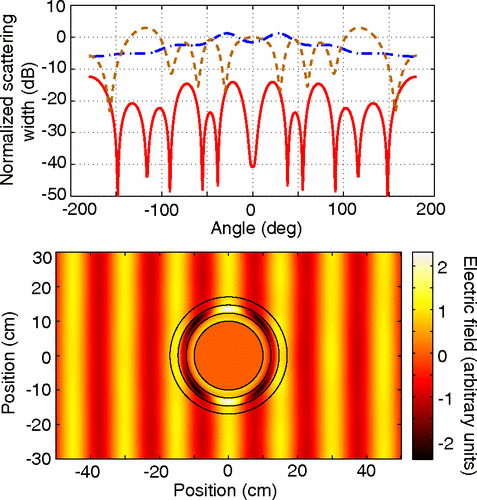
\includegraphics[height=0.4\paperheight, width=0.55\paperwidth]{fig4.png}
  \caption{}
  \label{fig:4}
\end{figure}

\end{document}
